\documentclass[journal]{IEEEtran}

\usepackage{graphicx}  %needed to include png, eps figures
\usepackage{float}  % used to fix location of images i.e.\begin{figure}[H]

\begin{document}

\title{ECSE 444 - Final Project Proposal (G21)}

\author{Christopher Ghosn, Qihao Wu, Zichen Gao, Nader Akel}

% make the title area
\maketitle

\section{Project Description}
Our project consists of a walkie talkie system that uses two or more boards to record and play audio signals that they send wirelessly between each other in real time. The features that will likely be used are the DFSDM microphone, the DAC speaker, either Bluetooth or WiFi, and likely the CMSIS DSP and UART.

The system will connect two or more boards wirelessly either through a WiFi or Bluetooth connection so that they can send data to each other. The on-board DFSDM microphone will be used to record audio. The audio signal will then be compressed using the CMSIS DSP functions so that it takes up less bandwidth, and will then be wirelessly transmitted to another board. The recevier board will then receive the signal, decompress it using the CMSIS DSP functions, and play it on a DAC microphone. UART will be used to output debug messages (send a text when boards are connected, when sound has been successfully received, etc.). The entire prcocess is shown in Fig. \ref{Diagram}.

\begin{figure}[H]
    \centering
    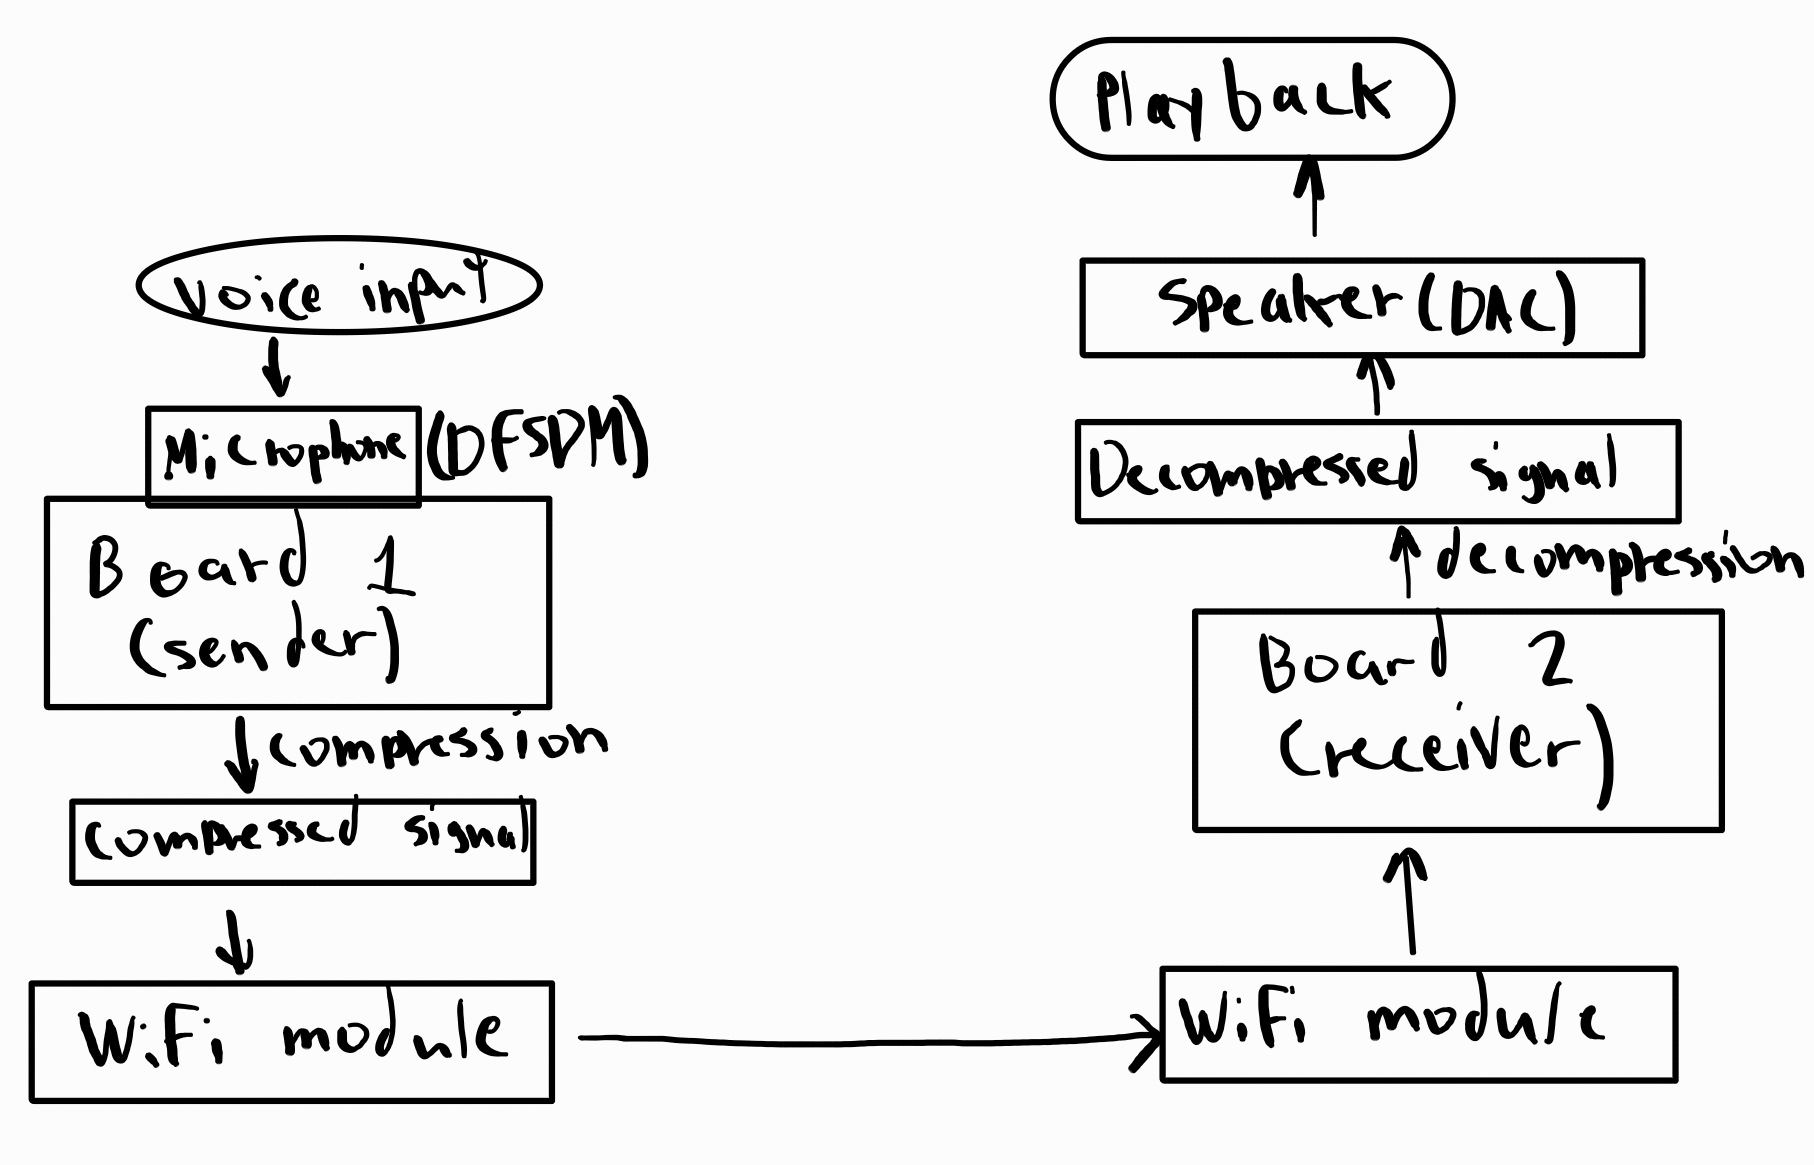
\includegraphics[width = 3in]{bibtex/Images/Diagram.png}
    \caption{Diagram of the walkie talkie system}
    \label{Diagram}
\end{figure}

\section{Milestones and Planned Timeline}
The first part of the project will be to get a reliable implementation of audio recording and playback on a board (by November 7th). We will then get to implement wireless data transfers through either WiFi or Bluetooth between two boards (by November 13th). After that, we will make a working implementation of the system that only works one-way (one board records sends and one board receives and plays) (by November 17th). Then, we will implement a method to compress the recorded audio signals and decompress them before playback so that less bandwidth can be used for data transfers and longer recordings can be made (by November 23rd). Finally, we will try to make the system work two-ways (and possibly with more than two boards in the network). We will also try making the boards work on a low-power mode when they are idle to consume less power if we have time for it.

We will use GitHub to be able to asynchronously work on the project. Qihao will be working on the audio recording and playback, Zichen on the wireless data transmission, Christopher on the processing and storage of the audio signals, and Nader on the system's procedures.

\section{Testing and Evaluation}
Our evaluation methodology is designed to be thorough, starting with individual sensor tests before moving on to the subsystems. The initial phase involves writing and executing code to assess the correct functionality of the microphone, DAC, and speaker. This will ensure that the components of our system are operating as intended. Once we have verified the performance of each sensor, we will proceed to evaluate the subsystems. This may be done in parallel where feasible, except in cases where the functionality of one subsystem is contingent upon another. This structured approach allows us to isolate and address specific issues that may arise. 

For subsystem testing, we will code to check voice collection, ensuring that the captured sound plays correctly through our DAC speaker. We will also test data transfer between boards and measure the rate if possible. Our next focus will be to evaluate the compression and decompression algorithms, which we are still currently researching, and determine how much compressed audio our storage can hold. Finally, we'll verify the speaker's output matches the input data and that playback works with a button press. This step-by-step testing ensures each subsystem works independently before full system integration.

After confirming that each subsystem is functioning properly, we will proceed with full system testing. This will involve checking the entire system's functionality and searching for edge cases to make sure our system is working under different conditions.

\end{document}